\subsection{Instrumentos de cuerda pulsada}
\label{c:fundamentos_cuerda}
Los \textbf{instrumentos de cuerda pulsada}~\cite{wikipedia_cuerdapulsada}, son aquellos que se tocan utilizando los dedos, las uñas o una púa. Podemos identificar dos elementos comunes:

\begin{itemize}
    \item Las \textbf{cuerdas}, normalmente nombradas con un índice comenzando por la derecha. Cada cuerda posee una \textbf{\gls{afinación}}, es decir, se le ha aplicado cierta tensión, de modo que seá capaz de reproducir una nota.
    \item Los \textbf{trastes}, unas tiras metálicas perpendiculares al mástil que, al igual que las cuerdas, reciben un nombre a modo de índice, comenzando desde arriba. Al presionar una cuerda sobre un traste se puede reproducir una nota más aguda a la afinada. Si tocamos la cuerda sin presionar ningún traste lo llamaremos \textbf{\gls{cuerda al aire}}.
\end{itemize}

La configuración de cuerdas y trastes \figref{fig:timple_partes} es equivalente a las teclas de un piano, es decir, si afinamos una cuerda en $Do$, los trastes bajo la misma serán equivalentes a las teclas de un piano comenzando en $Do$ \figref{fig:timple_notas_piano}

\begin{figure}[H]
    \centering
    \begin{subfigure}[t]{0.56\textwidth}
        \centering
        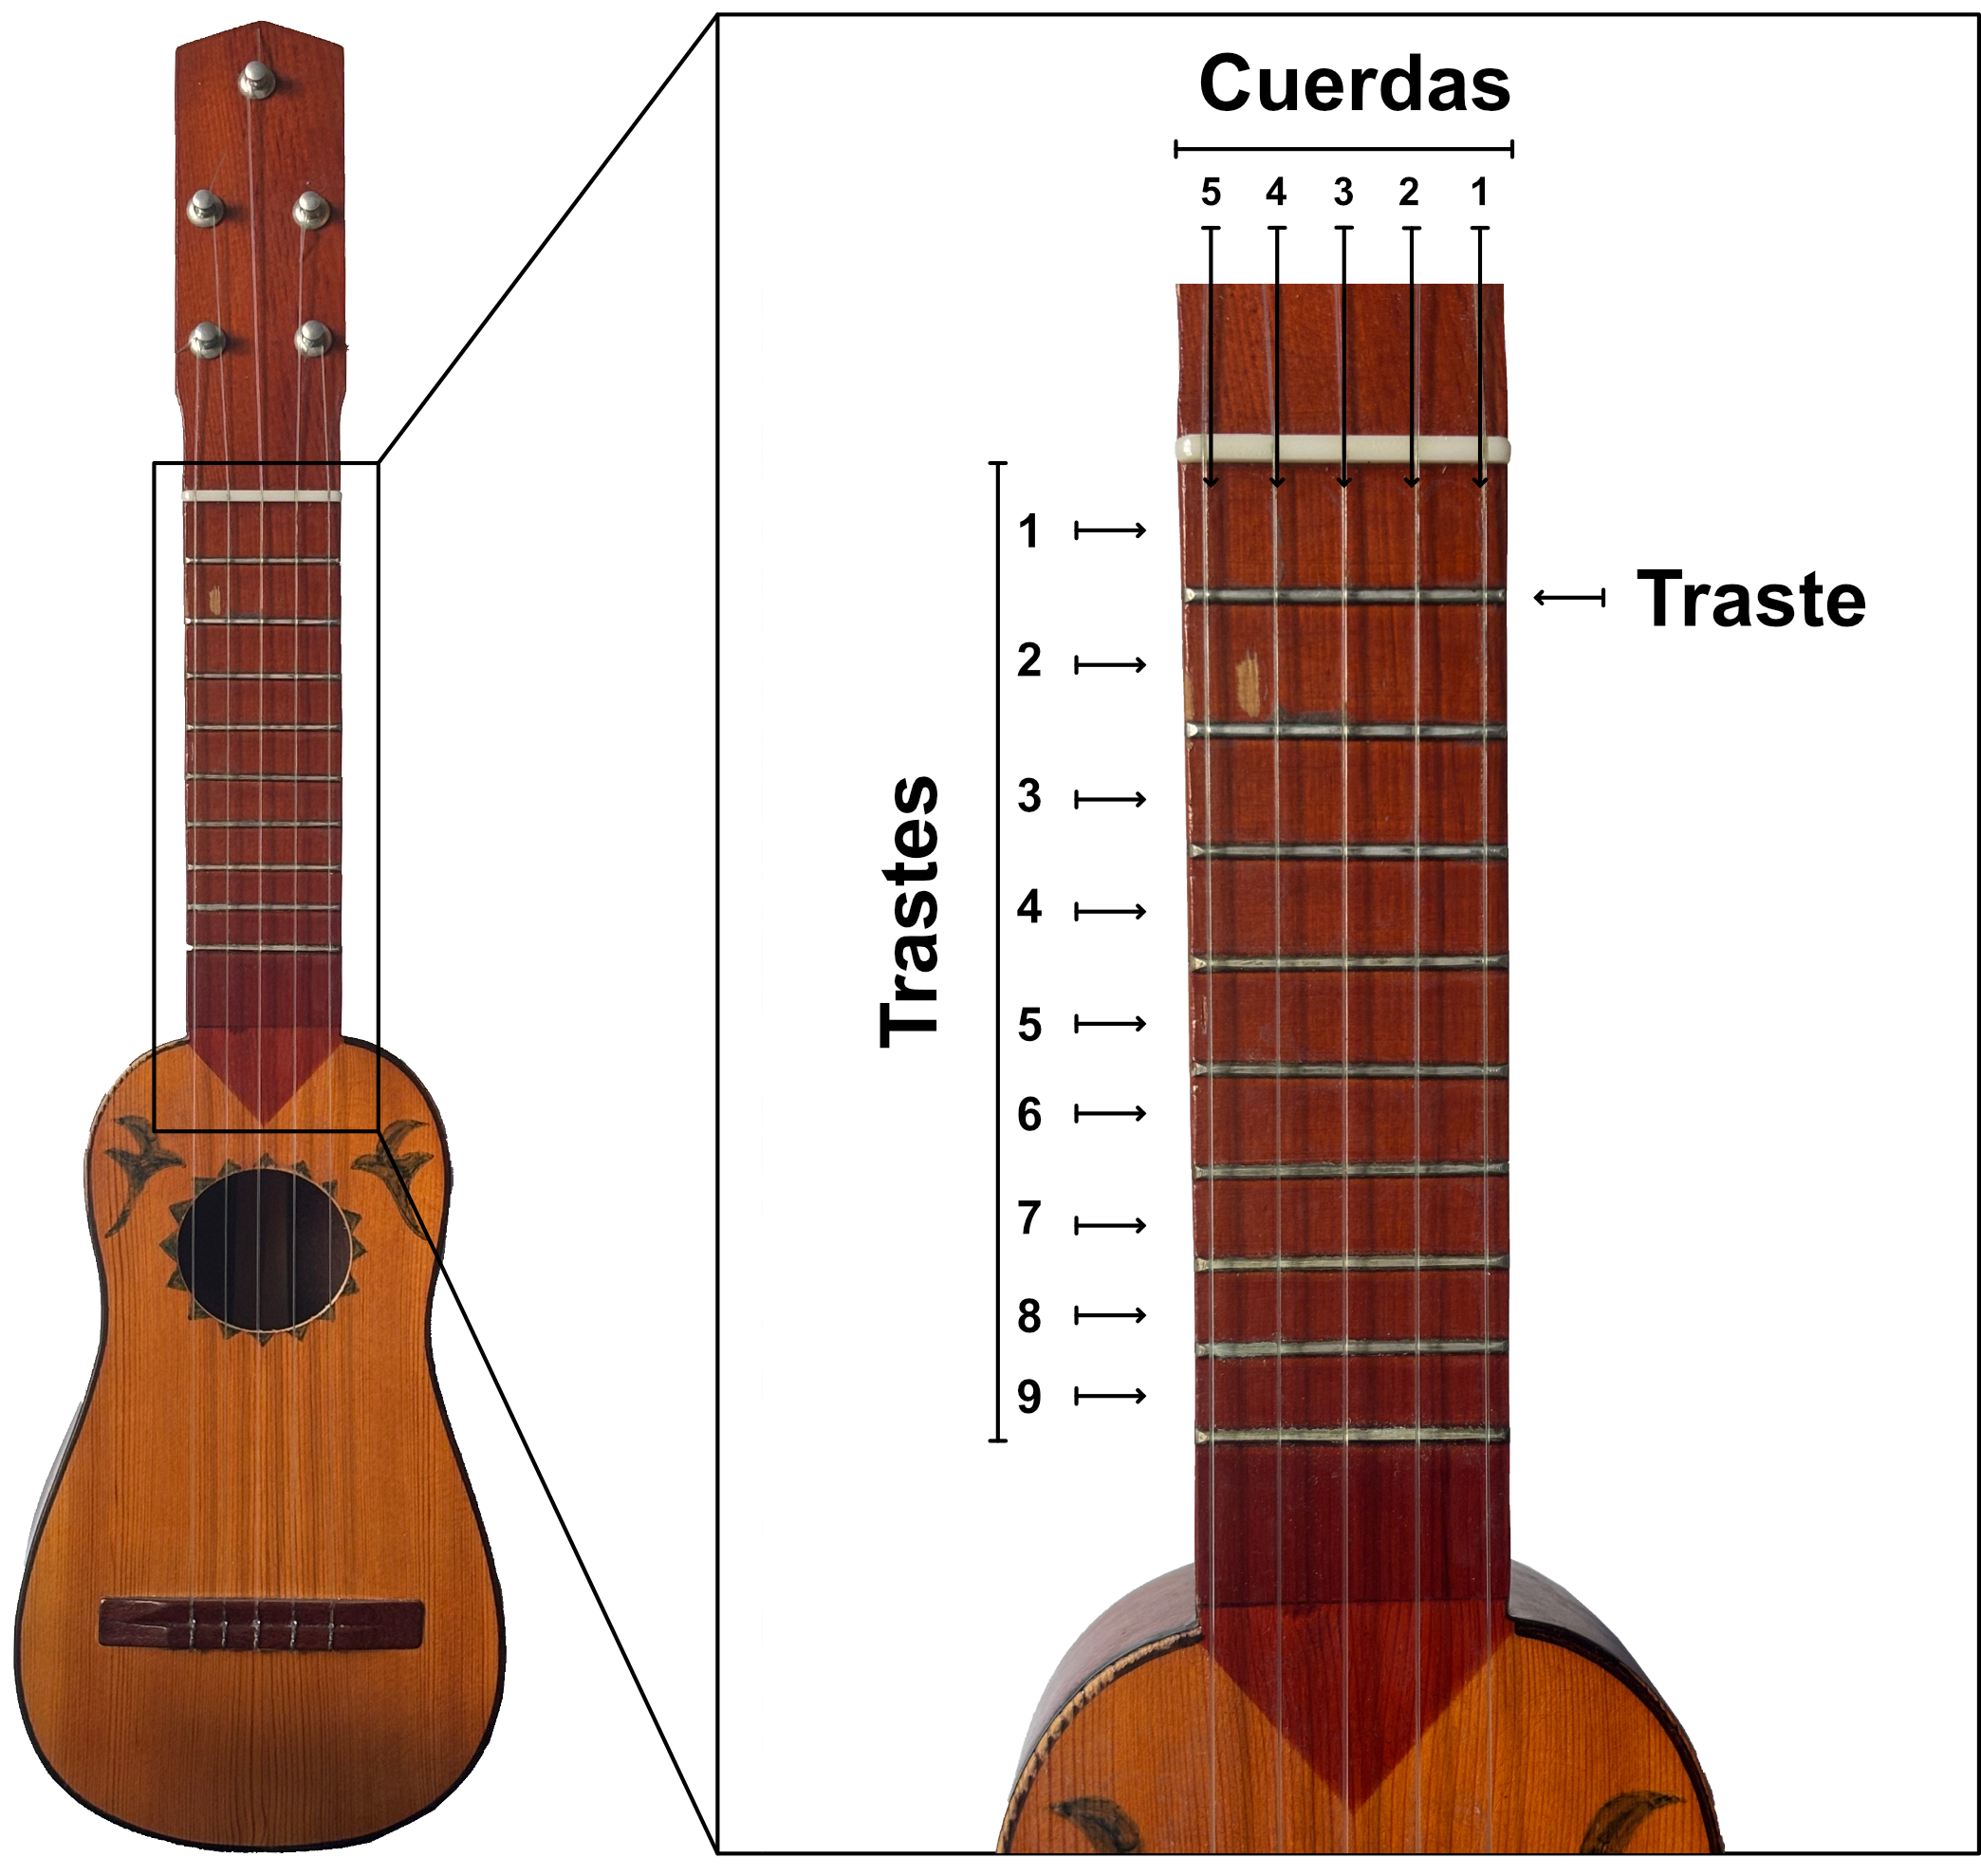
\includegraphics[width=\textwidth]{Ilustraciones/estado/timple_partes.jpg}
        \caption{Trastes y cuerdas en un timple}
        \label{fig:timple_partes}
    \end{subfigure}
    \hfill
    \begin{subfigure}[t]{0.40\textwidth}
        \centering
        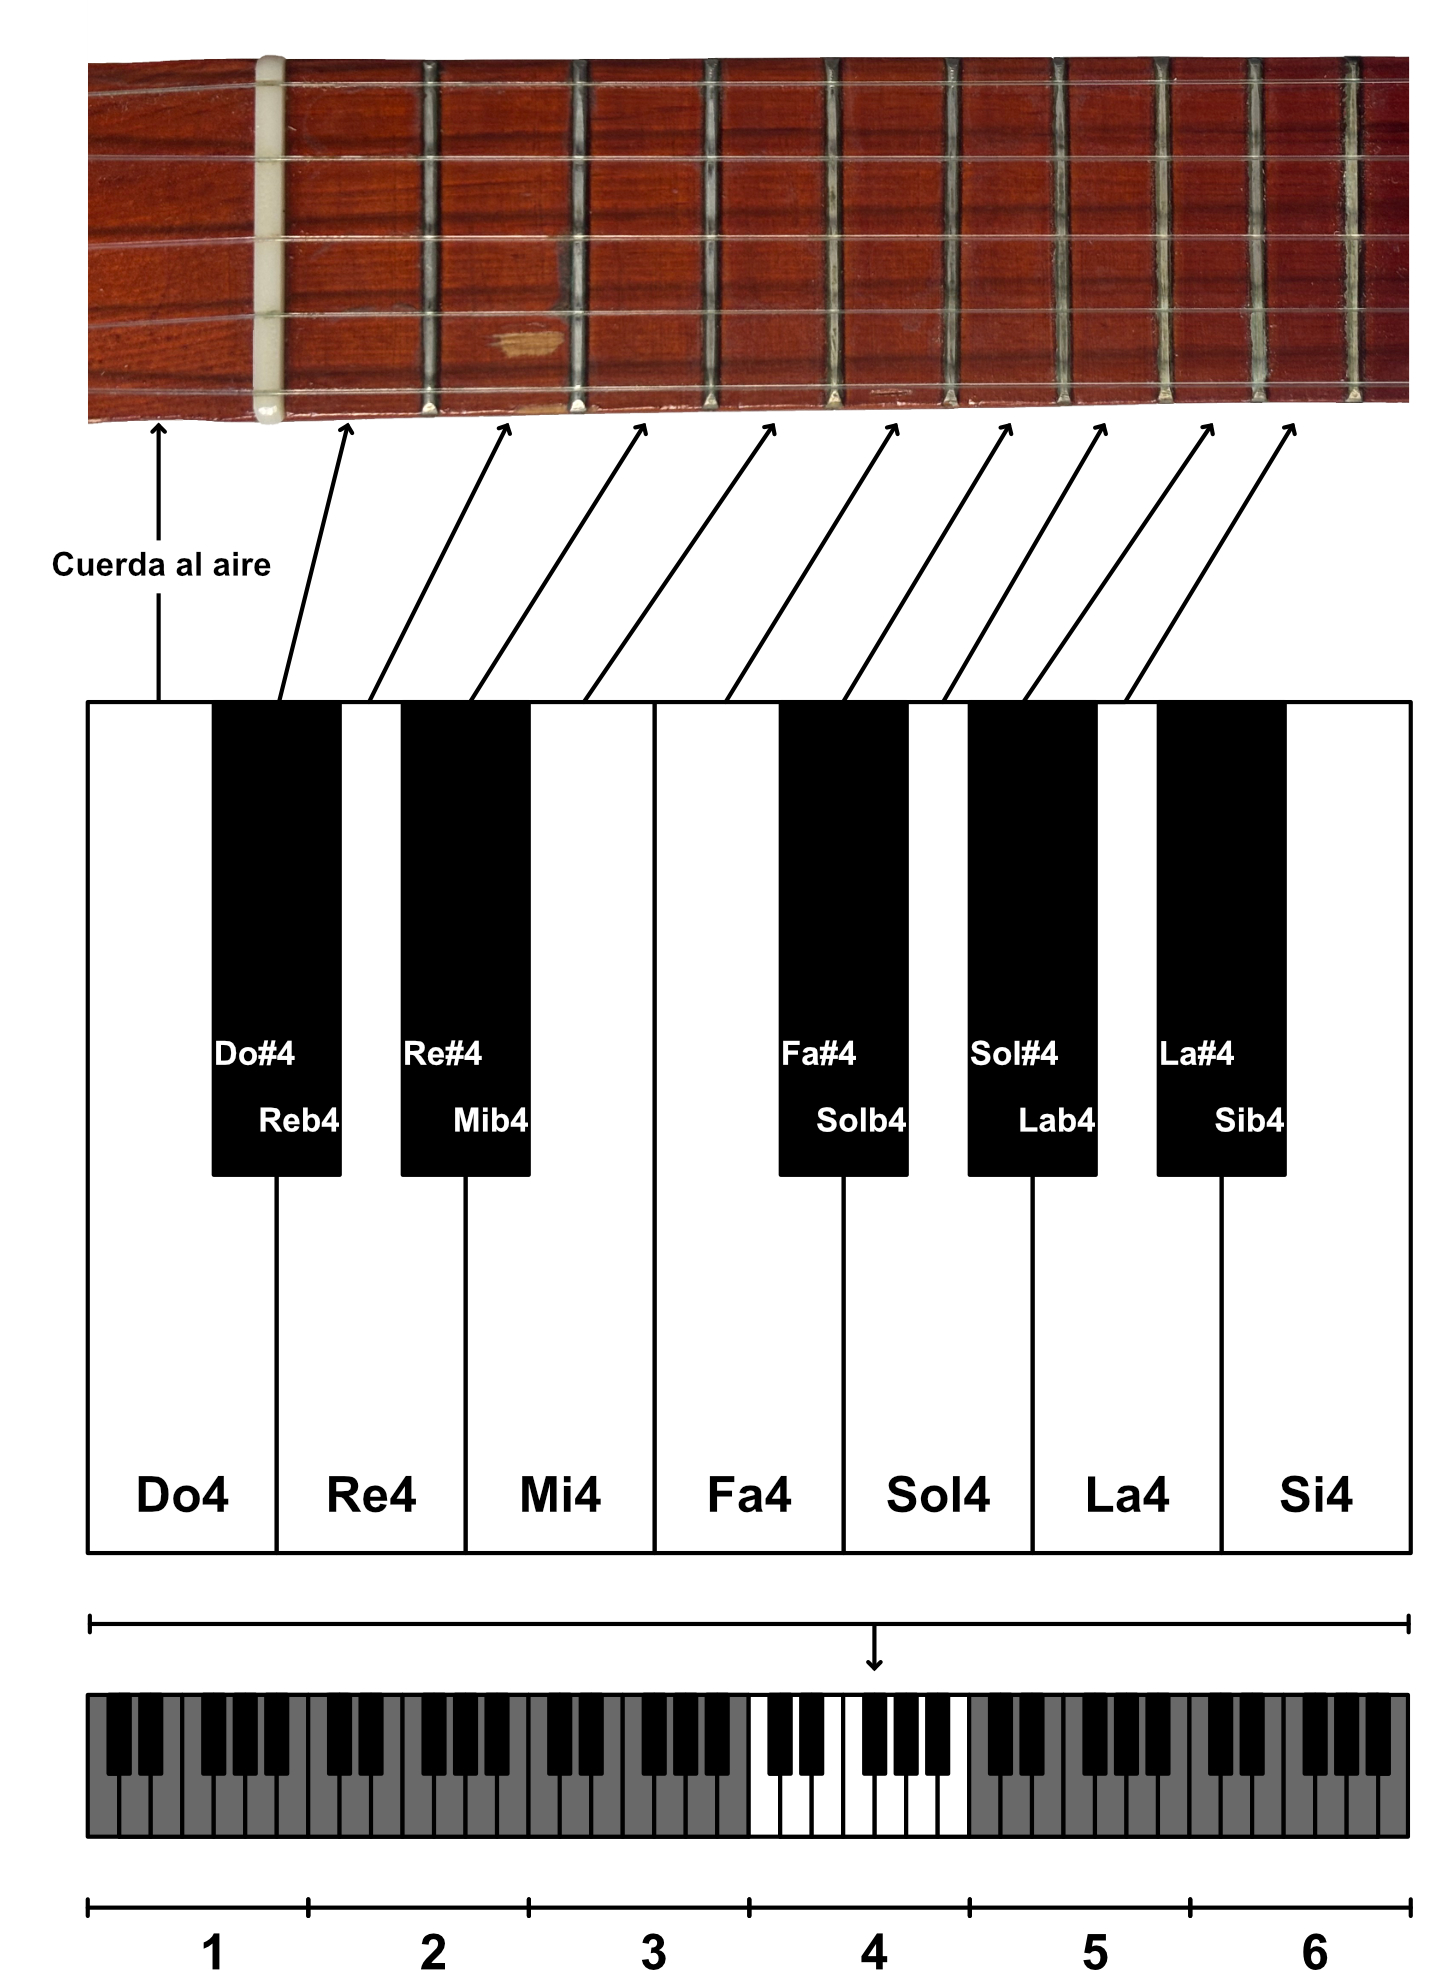
\includegraphics[width=\textwidth]{Ilustraciones/estado/timple_notas_piano.jpg}
        \caption{Relación entre notas del timple y el piano}
        \label{fig:timple_notas_piano}
    \end{subfigure}
    \caption{Comparación visual entre las partes del timple y su correspondencia con el piano.}
    \label{fig:timple_comparacion}
\end{figure}

Además, podemos instroducir el concepto \textbf{transposición de un instrumento}, que consiste en la transposición de todas las cuerdas al aire en un mismo número de semitonos.

Con respecto al toque de los instrumentos de cuerda pulsada, podemos distinguir dos técnicas:

\begin{itemize}
    \item El \textbf{\gls{punteo}}~\cite{wikipedia_punteo}, que consiste en el toque de notas individualmente.
    \item El \textbf{\gls{rasgueo}}~\cite{wikipedia_rasgueo}, que consiste en la reproducción de varias notas en forma de barrido, utilizando uno o mas dedos. Estos barridos se ejecutan siguiendo un patrón, existiendo una forma de representación a través de símbolos que indican la acción a ejecutar \tabref{tabla:simbolos_rasgueo}.
    \begin{table}[H]
        \centering
        \scriptsize
        \begin{tabular}{l c c c l}
            \hline
            \textbf{Rasgueo} & \multicolumn{3}{c}{\textbf{Símbolos}} & \textbf{Descripción} \\
            Abajo & $\downarrow$ & D & $\sqcap$ & Rasgueo hacia abajo (de cuerdas graves a agudas) \\
            Arriba & $\uparrow$ & U & $\vee$ & Rasgueo hacia arriba (de cuerdas agudas a graves) \\
            Percusión & $\times$ & $\times$ & $\times$ & Golpe de percusión o mute sobre la cuerda; se puede combinar con cualquier rasgueo \\
            \hline
        \end{tabular}
        \caption{Símbolos de rasgueo en instrumentos de cuerda pulsada}
        \label{tabla:simbolos_rasgueo}
    \end{table}
\end{itemize}

Finalmente, para la reproducción de canciones la notación en pentagrama es comunmente utilizada, pero existen ciertas notaciones diseñadas especificamente para este tipo de instrumentos:

\begin{itemize}
    \item La \textbf{\gls{tablatura}}~\cite{wikipedia_tablatura}, consiste en la representación gráfica de notas a través de una tabla \figref{fig:tablatura} donde cada linea horizontal equivale a una cuerda, los números equivalen a un traste y los simbolos indican efectos \tabref{tab:simbolos_tablatura}.
    
    \begin{table}[H]
        \centering
        \scriptsize
        \caption{Ejemplo de tablatura para timple}\label{fig:tablatura}
        \ttfamily
        \begin{tabular}{l l}
            Sol & |--0--2h--3--2--0-----------| \\
            Do  & |--2------------0-----------| \\
            Mi  & |--1------------2--2--2--2--| \\
            La  & |--2------------2-----------| \\
            Re  & |--0------------2-----------| \\
        \end{tabular}
    \end{table}

    \begin{table}[H]
        \centering
        \scriptsize
        \caption{Símbolos comunes de tablatura}\label{tab:simbolos_tablatura}
        \begin{tabular}{c l l}
            \hline
            \textbf{Símbolo} & \textbf{Nombre} & \textbf{Descripción} \\
            \hline
            h & Hammer & Se pulsa una nota martilleando con otro dedo sin volver a pulsar la cuerda \\
            p & Pull-off & Se suelta una nota dejando sonar una inferior ya pulsada \\
            / & Slide up & Deslizamiento hacia una nota más aguda \\
            \textbackslash & Slide down & Deslizamiento hacia una nota más grave \\
            b & Bend & Se estira la cuerda para subir la altura del sonido \\
            r & Release & Liberación del bend hacia la nota original \\
            $\sim$ & Vibrato & Pequeña oscilación continua en la nota \\
            t & Tapping & Percusión directa con un dedo de la mano derecha en el mástil \\
            \hline
        \end{tabular}
    \end{table}

    \item El \textbf{\gls{diagrama de acordes}}~\cite{imusicschool_diagramadeacordes}, consiste en la representación de los acordes a tocar sobre las palabras clave de la letra de una canción. Suele ir acompañado de una tabla donde las lineas verticales equivalen a las cuerdas y las horizontales a los trastes, utilizando circulos para indicar donde colocar los dedos~\figref{fig:diagrama_acordes}.
    
    \begin{figure}[H]
        \centering
        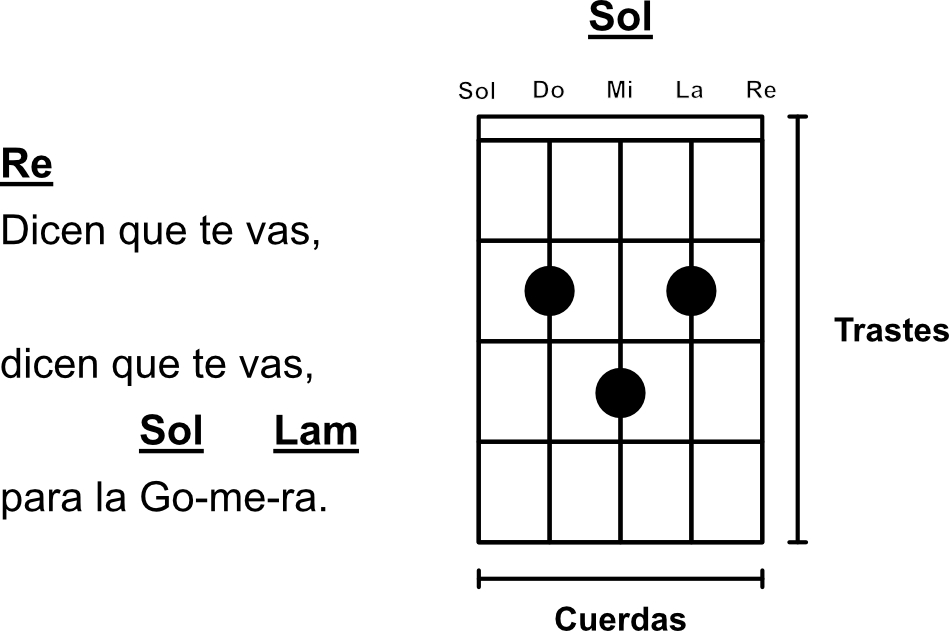
\includegraphics{Ilustraciones/estado/diagrama_acordes.jpg}
        \caption{Ejemplo de diagrama de acordes para timple}\label{fig:diagrama_acordes}
    \end{figure}
\end{itemize}